\def\documentType{Protocol}
\def\mainLanguage{ngerman}

\input{.template-locator.tex}

\pgfqkeys{/TemplateVersion0}{
	properties/Authors				= {Tom Mohr&&Martin Ohmeyer},
	properties/Title				= {Versuch V2},
	properties/Subtitle				= {C752 Digitaltechnik},
	properties/Institution			= {HTWK Leipzig},
	properties/Group				= {23INB-3},
	properties/Versioning			= {true},
	misc/Date/Prefix				= {Stand: },
	misc/Page/CountPrefix			= {Seiten: },
	misc/Group/Prefix				= {Gruppe: },
	Protocol/Comment				= {Abnahme: 16. Januar 2024}
}

\usepackage{minted}
\graphicspath{{./images/}}

\begin{document}
	\chapter{Aufgabe 3}
\section{Aufgabe 3.1}

\paragraph{Aufgabenstellung}
Sollten Sie bei den folgenden Punkten Wissenslücken feststellen, füllen Sie diese bitte vor dem Laborversuch selbstständig auf z.B. durch YouTube Videos.

\paragraph{Vorüberlegung}
Es bestehen keine größeren Defizite in den Gebieten \textit{RS232}, \textit{DMX}, \textit{ASCII} und \textit{Baudrate/Bitrate}.

\paragraph{Schlussfolgerung}
Der Wissensstand ist ausreichend, um die folgenden Aufgaben gewissenhaft erledigen zu können.
	
	%!TEX root = DT_V2_tom-mohr_martin-ohmeyer.tex
\chapter{Aufgabe 4}
\section{Aufgabe 4.1}
\paragraph{Aufgabenstellung}
Schließen Sie das Oszilloskop an den \textit{TXD} Ausgang des Arduinos an. Analysieren Sie das Signal.

\paragraph{Vorbereitung}
Um den Arduino verwenden zu können, benötigt er eine Betriebsspannung von \SI{5}{V}, welche das Netzteil bereitstellt. Der Arduino wird mit den Pins \textit{VIN} und \textit{GND} mit dem Netzteil verbunden. Bei dem verwendeten Protokoll gibt es (der Aufgabenstellung nach) zwei Möglichkeiten: \textit{DMX} und \textit{RS232}. Während \textit{DMX} differentiell übertragen wird, ist dies bei \textit{RS232} nicht der Fall. Bei manueller Auswertung des Signal ist beachten, dass das \textit{least significant bit (LSB)} zuerst und das \textit{most significant bit (MSB)} zuletzt übertragen wird. Das Signal muss also \glqq{}rückwärts\grqq{} gelesen werden. Nach Anweisung der Prüfer sollen nur die ersten drei Buchstaben konvertiert werden. Die nach der Auswertung erhaltenen Dezimalzahlen müssen mithilfe des ASCII-Standards konvertiert werden.

\paragraph{Durchführung}
Mit einem Trigger wird die Erfassung des Signals am Oszilloskop angehalten, damit dieses, wie in Abb. \vref{task4-1-img} abgelesen werden kann. Danach müssen die Hochs und Tiefs des Signal als 1 und 0 interpretiert werden. Die erhaltene Binärfolge lautet

\begin{equation*}
	\textcolor{ForestGreen}{0}\underbrace{00100010}_{68 \ \equiv \ D}\textcolor{red}{1}
	\textcolor{ForestGreen}{0}\underbrace{10000110}_{97 \ \equiv \ a}\textcolor{red}{1}
	\textcolor{ForestGreen}{0}\underbrace{11001110}_{115 \ \equiv \ s}\textcolor{red}{1}
\end{equation*}\\

\noindent und stellt die Buchstaben \glqq{}D\grqq{}, \glqq{}a\grqq{} und \glqq{}s\grqq{} dar \textit{(\textcolor{ForestGreen}{Grün} = Startbits, \textcolor{red}{Rot} = Stopbits)}. Die Baudrate errechnet sich mit dem Quotienten aus 1 und der Übertragungsdauer eines Bits:\\

\begin{tabular}{llll}
	\textbf{geg.:} & $f_s = 120 \mu s = 1,2 \times 10^{-4} s$      & \textbf{ges.:} & $T_s$ \\
	\textbf{Lsg:}  & $T_s = \frac{1s}{f_s}$                        &                &       \\
	               & $T_s = \frac{1s}{1,2 \times 10^{-4}s}$        &                &       \\
	               & $T_s = \SI{8333,3}{Bd} \approx \SI{8,3}{kBd}$ &                &
\end{tabular}

\paragraph{Schlussfolgerung}
Das übertragene Signal nicht differentiell, weswegen es sich bei dem Protokoll um \textit{RS232} handeln muss. Es wird ein einzelnes Stopbit verwendet, welches 1 ist. Die Baudrate beträgt \SI{8,3}{kBd}. Mögliche Fehler bei der Übertragung wären durch Paritätsbits sichtbar geworden, jedoch wurden diese nicht eingesetzt. Daher war eine Fehlerüberprüfung nicht möglich. Die Übertragung liefert das Wort \glqq{}Das\grqq{}.

\begin{figure}[!h]
	\centering
	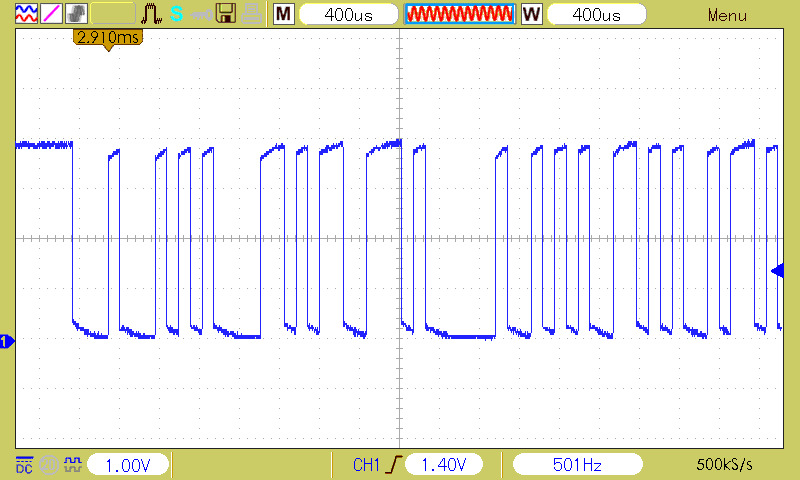
\includegraphics[width=.7\textwidth]{task4-1.jpg}
	\caption{Beginn des RS232 Signals}
	\label{task4-1-img}
\end{figure}

\section{Aufgabe 4.2}
\paragraph{Aufgabenstellung}
Schließen Sie das Oszilloskop an die D+ und D- Pins des DMX-Boards an. Nutzen Sie die Mathematikfunktion um das Differenzsignal darzustellen.

\paragraph{Vorteile der differentiellen Signalübertragung}
Die differentielle Signalübertragung wird in allen modernen Protokollen verwendet. Fast alle Bussysteme, die außerhalb eines Gerätes liegen, greifen auf sie zurück. Ihre Stärke liegt in einer hohen Fehlerresistenz auch bei niedrigen Spannungen, was schnelle Übertragungsraten ermöglicht. Die Übertragung eines differenziellen Signals erfolgt dazu über zwei Kabel. Während das eine Kabel positive Spannungsausschläge verwendet, überträgt das andere Kabel negative des gleichen Betrages. Das ursprüngliche Signal wird dann durch Subtraktion der beiden einzelnen Spannungen errechnet. Der große Vorteil: Verdrillt man die beiden Kabel, so wirkt eine Störung von außen auf beide gleichermaßen. Zwar ändern sich die Spannungsausschläge, welche durch die jeweiligen Kabel übertragen werden, ihre Differenz bleibt jedoch unberührt und die übermittelten Daten unbeschädigt.

\paragraph{Durchführung}
Das Oszilloskop subtrahiert beide vom DMX-Board kommende Signale voneinander, sodass dabei das in Abb. \vref{task4-2-img} differentielle Signal als grüne Welle dargestellt wird.

\begin{figure}[!h]
	\centering
	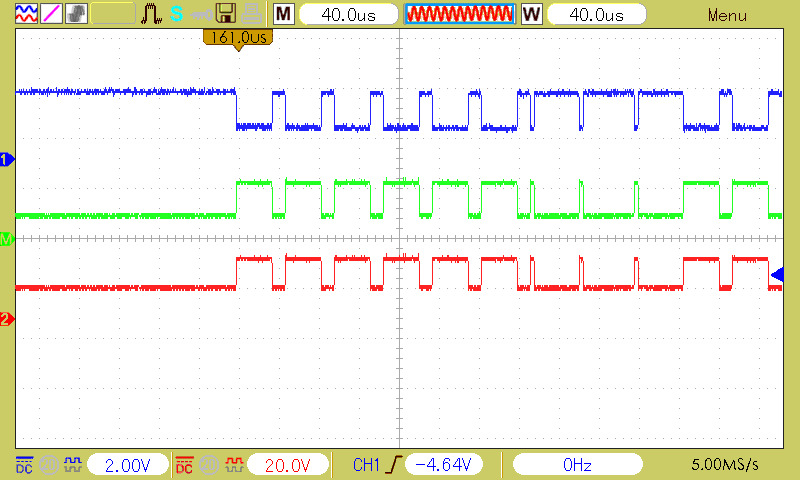
\includegraphics[width=.6\textwidth]{task4-2.jpg}
	\caption{Differentielle Signalübertragung}
	\label{task4-2-img}
\end{figure}

\paragraph{Schlussfolgerung}
Die Baudrate beträgt \SI{31205}{Bd}.

\section{Aufgabe 4.3}
\paragraph{Aufgabenstellung}
Benutzen Sie den Logicanalyser um das Zitat zu dekodieren welches der RS232-Arduino sendet.

\paragraph{Vorbereitung}
Der Pinbelegung des Logicanalyser nach, wird dieser mit dem Arduino über \textit{D0} und \textit{GND} verbunden. Um die Messwerte auszuwerten kann das Programm \textit{Pulsview} verwendet werden. Die Abtatsrate des Signals müssen höher sein, als die der gesendeten Daten, um verlustfreie Ergebnisse zu erhalten

\paragraph{Durchführung}
Das Programm wird mit dem Typ des Logicanalysers, \SI{5}{M Samples} und \SI{1}{Mhz} konfiguriert. Der Kanal 0 wird mittels \textit{UART} und der Baudrate aus Aufgabe 4.1 ausgewertet. Die Auswertung bestätigt alle Annahmen aus Aufgabe 4.1, dass keine Paritätsbits vorhanden sind und ein Stopbit zu verwendet wird.

\paragraph{Schlussfolgerung}
Das übertragene Zitat lautet:
\begin{quote}
	Das einzig sichere System müsste ausgeschaltet, in einem versiegelten und von Stahlbeton ummantelten Raum und von bewaffneten Schutztruppen umstellt sein. Gene Spafford - Sicherheitsexperte
\end{quote}


%!TEX root = DT_V2_tom-mohr_martin-ohmeyer.tex
\section{Aufgabe 4.4}
\paragraph{Aufgabenstellung}
Wählen Sie ein Musikstück aus und programmieren Sie für die ersten 30s die Beleuchtungssequenz.

\paragraph{Vorüberlegung}
Um die DMX-Geräte ansteuern zu können, wird eine Klasse bereitgestellt, welche man mit einer einfachen Funktion, der man Adresse und gewünschten DMX-Werte gibt, bedienen kann. Da die Geräte nur an einem Ort erreichbar sind, sollte das Programm während der Entwicklung auch mit lokalen LEDs an den Pins des Arduinos ausführbar sein und einen schnellen Wechsel zwischen Test- \& Produktionsmodus ermöglichen, ohne den Code in großem Umfang abändern zu müssen. Um dies zu realisieren, werden Klassen mit Polymorphismus benötigt. Da die Geräte ihre Befehle selbstständig abarbeiten sollen, kann hier nicht mit der Delay-Funktion des Arduinos gearbeitet werden. Ein anderer Ansatz ist, fortlaufend die verstrichene Zeit ermitteln und die Objekte selbst entscheiden lassen, wann sie ihre Befehle anführen.

\paragraph{Durchführung}
In der Hauptdatei werden die Geräte als Objekte initialisiert, das DMX-Interface vorbereitet und in einer Endlosschleife die Objekte aufgerufen um ihre Befehle abzuarbeiten.
\inputminted[linenos=true, breaklines, fontsize=\fontsize{10pt}{10pt}]{cpp}{../src/main.cpp}

Damit die Geräte später einheitlich angesteuert werden können und eine gleiche Befehlsstruktur verwenden, definiert \textit{DmxCommand} die Befehle. Jeder Befehl enthält einen Zeitstempel, den Kanal und welchen Wert dieser annehmen soll.
\inputminted[linenos=true, breaklines, fontsize=\fontsize{10pt}{10pt}]{cpp}{../src/DmxCommand.h}

Um dem Polymorphismus gerecht zu werden, wird eine Basisklasse benötigt. Von \textit{DmxDevice} erben die Klassen für Scheinwerfer und Movingheads mit einer Grundstruktur von Funktionen und Variablen.
\inputminted[linenos=true, breaklines, fontsize=\fontsize{10pt}{10pt}]{cpp}{../src/DmxDevice.h}

Von dieser Basisklasse kann nun die Klasse RgbwSpotlight8Ch für die Spotlichter erben, ihre Befehle definieren und Funktionen erweitern.
\inputminted[linenos=true, breaklines, fontsize=\fontsize{10pt}{10pt}]{cpp}{../src/RgbwSpotlight8Ch.h}

Damit im Testmodus statt den Scheinwerfern LEDs verwendet werden können, erbt eine weitere Klasse \textit{RgbwSpotlight8ChDemo} von \textit{RgbwSpotlight8Ch}, um das DMX-Interface lokal emulieren zu können.
\inputminted[linenos=true, breaklines, fontsize=\fontsize{10pt}{10pt}]{cpp}{../src/RgbwSpotlight8ChDemo.h}

\paragraph{Schlussfolgerung}
Zur Kompilierzeit wird festgelegt, ob sich das Programm im Test- oder Produktionsmodus befindet. Objekte aus Klassen können in beiden Modi gleich angesteuert werden, was das testen von Befehlen stark vereinfacht. Das Programm lässt die Geräte in einer Endlosschleife selbstständig ihre Befehle abarbeiten, ohne dass diese sich durch Verzögerungen blockieren. Der Versuch ist erfolgreich.



\newpage
\section{Aufgabe 4.5}
\paragraph{Aufgabenstellung}
Bitte räumen Sie auf und setzen Sie ggf. veränderte Arduinos zurück.

\paragraph{Durchführung}
Mithilfe des Befehls wird der Arduino zurückgesetzt:

\inputminted[breaklines, fontsize=\fontsize{10pt}{10pt}]{bash}{../docs/reset-dmx.txt}

\paragraph{Schlussfolgerung}
Der Arduino befindet sich in seinem Ausgangszustand und wurden Ordnungsgemäß zurück geräumt.
\end{document}